\documentclass{beamer}
\usepackage[utf8]{inputenc}
\usepackage{amsmath,amssymb}
\usepackage{booktabs}
\usepackage{array}
\usepackage{tikz}
\usetikzlibrary{arrows.meta,positioning,shapes.geometric}

\usetheme{Madrid}
\usecolortheme{default}

%------------------------------------------------------------
% Title Page Configuration
%------------------------------------------------------------
\title[RehabOpt-AR] % Short title for footer
{RehabOpt-AR: Vision-Based AR Telerehabilitation System for Upper-Limb Stroke Recovery}

\subtitle{Markerless Computer Vision, Kinematic Anti-Cheat Engine, \& Clinical Protocol}

\author[Group 12]
{Athul V R~(CB.AI.U4AID25005) \and
 T.V.S.S. Phanindra Gupta~(CB.AI.U4AID25055) \and
 M. Vittal~(CB.AI.U4AID25033) \and
 K. Nanda Kishore~(CB.AI.U4AID25027)}

\institute[Amrita Vishwa Vidyapeetham]
{
  Department of Artificial Intelligence\\
  Amrita School of Artificial Intelligence, Coimbatore\\
  Amrita Vishwa Vidyapeetham, India
}

\date[Project Review 2026]{Final Project Presentation, October 2026}

% Remove navigation symbols for cleaner slides
\setbeamertemplate{navigation symbols}{}

%------------------------------------------------------------
% Table of Contents at the beginning of each section
%------------------------------------------------------------
\AtBeginSection[]
{
  \begin{frame}
    \frametitle{Table of Contents}
    \tableofcontents[currentsection]
  \end{frame}
}

%------------------------------------------------------------
\begin{document}

% Slide 1: Title
\frame{\titlepage}

% Slide 2: Table of Contents
\begin{frame}
\frametitle{Presentation Outline}
\tableofcontents
\end{frame}

%============================================================
\section{Introduction \& Clinical Motivation}
%============================================================

\begin{frame}{Clinical Motivation \& Background}
\begin{columns}
\column{0.55\textwidth}
\begin{itemize}
    \item \textbf{Global Stroke Burden}: Stroke is the leading cause of adult long-term motor disability worldwide.
    \item \textbf{Upper-Limb Impairment}: Up to 80\% of acute stroke survivors suffer hemiparesis or loss of arm/hand motor control.
    \item \textbf{Neuroplasticity Window}: Motor recovery strictly demands high-repetition, consistent, goal-oriented daily training.
    \item \textbf{Clinic Bottlenecks}:
    \begin{itemize}
        \item High clinic therapy costs and transportation barriers.
        \item Poor patient adherence ($<30\%$) with unsupervised paper sheets.
        \item Lack of objective biomechanical progress tracking.
    \end{itemize}
\end{itemize}

\column{0.45\textwidth}
\begin{alertblock}{The Problem in Existing AR/Apps}
\begin{itemize}
    \item \textbf{Hardware Dependency}: Require expensive VR headsets or wearable IMU sensors.
    \item \textbf{Cheating / Compensation}: Patients lean their trunk instead of moving their arm.
    \item \textbf{Shallow Reps}: Patients swing arms without reaching true functional range.
\end{itemize}
\end{alertblock}
\end{columns}
\end{frame}

\begin{frame}{Problem Statement \& Research Objectives}
\begin{block}{Problem Statement}
Develop a 100\% markerless, hardware-free Augmented Reality telerehabilitation platform using standard commodity webcams that enforces clinically valid range-of-motion, prevents compensatory cheating, and automates real-time rep counting.
\end{block}

\vspace{2mm}
\begin{columns}
\column{0.5\textwidth}
\textbf{Key Objectives}:
\begin{enumerate}
    \item \textbf{Zero-Sensor Tracking}: MediaPipe Pose + 21 Hand mesh running at 60 FPS in browser.
    \item \textbf{Anti-Cheat Kinematics}: Real-time trunk tilt compensation lockout ($>25^\circ$).
    \item \textbf{Two-Phase Rep Counting}: 0.5 Half-Rep on isometric target hold + 1.0 Full-Rep on controlled return.
\end{enumerate}

\column{0.5\textwidth}
\begin{enumerate}
    \setcounter{enumi}{3}
    \item \textbf{Comprehensive Clinical Suite}:
    \begin{itemize}
        \item 9 Clinical Exercise Drills.
        \item 7 ADL (Daily Living) Task Simulations.
        \item 4 Gamified Neuro-Arcade Games.
        \item Air-Canvas Neon Drawing Therapy.
    \end{itemize}
    \item \textbf{Clinical Portal}: HIPAA/GDPR-compliant clinician telemetry \& analytics.
\end{enumerate}
\end{columns}
\end{frame}

%============================================================
\section{System Architecture \& Engineering}
%============================================================

\begin{frame}{High-Level System Architecture}
\begin{center}
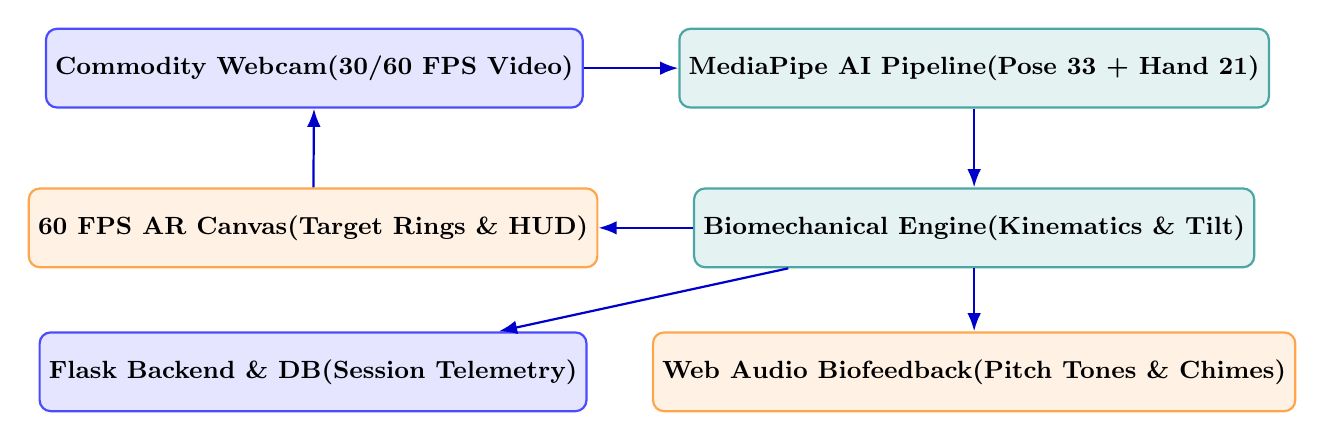
\begin{tikzpicture}[
    box/.style={rectangle, draw=blue!70, fill=blue!10, rounded corners, thick, text centered, minimum width=2.8cm, minimum height=1cm, font=\small\bfseries},
    proc/.style={rectangle, draw=teal!70, fill=teal!10, rounded corners, thick, text centered, minimum width=2.8cm, minimum height=1cm, font=\small\bfseries},
    ar/.style={rectangle, draw=orange!70, fill=orange!10, rounded corners, thick, text centered, minimum width=2.8cm, minimum height=1cm, font=\small\bfseries},
    arrow/.style={-Latex, thick, blue!80!black}
]
    \node (cam) [box] {Commodity Webcam\\(30/60 FPS Video)};
    \node (vision) [proc, right=1.2cm of cam] {MediaPipe AI Pipeline\\(Pose 33 + Hand 21)};
    \node (engine) [proc, below=1.0cm of vision] {Biomechanical Engine\\(Kinematics \& Tilt)};
    \node (arbox) [ar, left=1.2cm of engine] {60 FPS AR Canvas\\(Target Rings \& HUD)};
    \node (bio) [ar, below=0.8cm of engine] {Web Audio Biofeedback\\(Pitch Tones \& Chimes)};
    \node (backend) [box, below=0.8cm of arbox] {Flask Backend \& DB\\(Session Telemetry)};

    \draw [arrow] (cam) -- (vision);
    \draw [arrow] (vision) -- (engine);
    \draw [arrow] (engine) -- (arbox);
    \draw [arrow] (engine) -- (bio);
    \draw [arrow] (engine) -- (backend);
    \draw [arrow] (arbox) -- (cam);
\end{tikzpicture}
\end{center}
\begin{itemize}
    \item \textbf{Client-Side Edge AI}: All computer vision runs locally via WebAssembly/WebGL with 0 ms server video latency.
    \item \textbf{Privacy by Design}: Raw video frames never leave patient hardware; only numeric joint kinematics are stored.
\end{itemize}
\end{frame}

\begin{frame}{Biomechanical Kinematics \& Anti-Cheat Engine}
\begin{columns}
\column{0.5\textwidth}
\begin{block}{Joint Angle Formulation}
Joint angles $\theta$ at elbow and shoulder are evaluated via dot-product Euclidean vectors:
$$\theta = \arccos\left(\frac{\vec{v}_{1} \cdot \vec{v}_{2}}{\|\vec{v}_{1}\| \|\vec{v}_{2}\|}\right) \times \frac{180^\circ}{\pi}$$
Where $\vec{v}_1 = \vec{P}_{\text{shoulder}} - \vec{P}_{\text{elbow}}$ and $\vec{v}_2 = \vec{P}_{\text{wrist}} - \vec{P}_{\text{elbow}}$.
\end{block}

\begin{block}{Hand Spasticity / Spread Metric}
$$\text{Spread Ratio} = \frac{\frac{1}{5}\sum_{i \in \{4,8,12,16,20\}} \|\vec{P}_i - \vec{P}_{\text{palm}}\|}{\|\vec{P}_9 - \vec{P}_0\|}$$
Scale-invariant ratio normalizes across children and adults.
\end{block}

\column{0.5\textwidth}
\begin{alertblock}{Anti-Cheat Trunk Tilt Filter}
$$\text{Tilt Angle} = \left| \arctan2(\Delta y_{\text{shoulders}}, \Delta x_{\text{shoulders}}) \right| \times \frac{180^\circ}{\pi}$$
\begin{itemize}
    \item \textbf{Compensation Lock}: If trunk leans $>25^\circ$, exercise freezes with audio alert: \textit{"Posture cheat detected: keep shoulders level."}
    \item \textbf{Contextual Exemption}: Shoulder shrugs naturally tilt the inter-shoulder line; dynamically exempted to allow genuine shrugs!
\end{itemize}
\end{alertblock}
\end{columns}
\end{frame}

%============================================================
\section{The 9 Clinical Rehabilitation Exercises}
%============================================================

\begin{frame}{Two-Phase Clinical Rep Counting Logic}
\begin{block}{Why Two-Phase Counting (0.5 Half-Rep $\rightarrow$ 1.0 Full-Rep)?}
In stroke recovery, swinging an arm quickly without isometric control builds zero neuromuscular strength. RehabOpt-AR enforces genuine therapeutic movement:
\end{block}

\vspace{3mm}
\begin{columns}
\column{0.5\textwidth}
\begin{goodblock}
\begin{block}{Phase 1: Target Reach (0.5 Rep)}
\begin{itemize}
    \item Patient extends joint to reach clinical threshold (e.g., $\ge 140^\circ$).
    \item Must hold wrist/joint inside target for isometric hold duration (0.4s – 1.2s).
    \item \textbf{Audio Ding + Badge}: \textit{"Half Rep (0.5) Complete!"}
\end{itemize}
\end{block}
\end{goodblock}

\column{0.5\textwidth}
\begin{block}{Phase 2: Controlled Return (1.0 Rep)}
\begin{itemize}
    \item Patient performs eccentric controlled return back to resting posture (e.g., $< 125^\circ$).
    \item Prevents spastic dropping of the arm.
    \item \textbf{Chime + Fanfare}: \textit{"Repetition Complete!"} Counter increments $N / 10$.
\end{itemize}
\end{block}
\end{columns}
\end{frame}

\begin{frame}{Clinical Protocol: Exercises 1 to 5}
\begin{table}[]
\centering
\small
\begin{tabular}{lp{3.5cm}p{3.5cm}c}
\toprule
\textbf{Ex} & \textbf{Exercise Name} & \textbf{Clinical Thresholds} & \textbf{Hold} \\
\midrule
\textbf{1} & Elbow Extension \& Flexion & Angle $\ge 140^\circ$ + Corner Target $\rightarrow$ Flex $< 125^\circ$ & 0.6s \\
\textbf{2} & Shoulder Elevation (Shrug) & Shrug lift $\ge 3.5\%$ screen $\rightarrow$ Relax to resting baseline & 1.2s \\
\textbf{3} & Hand Open \& Close & Clench tight fist ✊ $\rightarrow$ Wide open palm 🖐️ & 0.4s / 0.5s \\
\textbf{4} & Horizontal Wrist Up/Down & Cock wrist UP $\ge 14^\circ$ $\rightarrow$ Return to level $\le 10^\circ$ & 0.5s \\
\textbf{5} & Diagonal Reach \& Hold & Reach diagonal target + maintain steady hold & 2.0s \\
\bottomrule
\end{tabular}
\end{table}
\begin{itemize}
    \item \textbf{Adaptive Target Placement}: Automatically mirrors depending on whether left or right arm is exercised.
\end{itemize}
\end{frame}

\begin{frame}{Clinical Protocol: Exercises 6 to 9}
\begin{table}[]
\centering
\small
\begin{tabular}{lp{3.5cm}p{3.5cm}c}
\toprule
\textbf{Ex} & \textbf{Exercise Name} & \textbf{Clinical Thresholds} & \textbf{Hold} \\
\midrule
\textbf{6} & Two-Target Horizontal Glide & Glide wrist to S2 (Right) $\rightarrow$ Return to S1 (Left) & 0.6s / 0.6s \\
\textbf{7} & Open Palm L/R Rotation & Knuckle lateral shift $<-0.035$ (Left) $\rightarrow$ $>0.035$ (Right) & 0.4s / 0.4s \\
\textbf{8} & Dynamic Moving Target Pursuit & Sinusoidal gliding target orb; wrist inside for 10s countdown & 10.0s \\
\textbf{9} & Virtual Pincer Grasp \& Release & Pinch Thumb-Index ($\le 0.32$) $\rightarrow$ Release wide open ($\ge 0.40$) & 0.5s \\
\bottomrule
\end{tabular}
\end{table}

\begin{block}{Exercise 8: Dynamic Moving Target Pursuit}
\begin{itemize}
    \item Target orb moves along smooth trajectory: $X(t) = 0.50 + 0.28\sin(0.65t)$, $Y(t) = 0.48 + 0.08\sin(1.3t)$.
    \item Live reverse countdown: counts down while wrist is inside target; resets back if wrist leaves outside for $>450$ ms.
\end{itemize}
\end{block}
\end{frame}

\begin{frame}{High-Visibility AR Overlay Interface}
\begin{columns}
\column{0.5\textwidth}
\textbf{60 FPS AR Canvas Rendering}:
\begin{itemize}
    \item \textbf{Concentric Target Rings}: Inner bullseye, crosshairs, and outer pulsating radar waves.
    \item \textbf{Circular Hold Gauge}: Radial green progress arc fills smoothly as hold duration progresses.
    \item \textbf{Live Skeletal Overlay}:
    \begin{itemize}
        \item Green bones (\#00C853) with yellow joint tags.
        \item Floating live degree readout (e.g., $\theta = 145^\circ$).
        \item 21 red hand landmarks with fingertip targeting halo.
    \end{itemize}
\end{itemize}

\column{0.5\textwidth}
\begin{exampleblock}{Tolerant Jitter Handling}
\begin{itemize}
    \item \textbf{300ms Hold Grace Window}: MediaPipe frame drops during rapid movement do not reset patient hold progress to 0.
    \item \textbf{Non-Blocking HUD}: Floating guidance cards docked at bottom leave video workspace 100\% unobstructed.
\end{itemize}
\end{exampleblock}
\end{columns}
\end{frame}

%============================================================
\section{ADL Lab, Arcade Arena, \& Gamification}
%============================================================

\begin{frame}{ADL Lab: Real-World Functional Simulation}
\begin{columns}
\column{0.5\textwidth}
\textbf{7 Daily Living Tasks}:
\begin{enumerate}
    \item \textbf{Balloon Pump}: Open hand to grasp pump, clench fist to compress air, inflate and pop.
    \item \textbf{Water Reservoir}: Transfer water between 4 tanks with cupped palm.
    \item \textbf{Light Switch}: Ballistic upward wrist flick to illuminate room.
    \item \textbf{ATM PIN Pad}: Index fingertip targeting with 90px sticky hit-boxes.
\end{enumerate}

\column{0.5\textwidth}
\begin{enumerate}
    \setcounter{enumi}{4}
    \item \textbf{Pour the Water}: Forearm pronation tilt tracking liquid flow volume.
    \item \textbf{Cup Shelf Lift}: Grasp cup, anti-gravity vertical elevation, placement on shelf.
    \item \textbf{Clean Window Dust}: Index scrubbing coverage reaching $\ge 90\%$ surface dust removal.
\end{enumerate}

\begin{block}{Clinical Value}
Bridges the gap between clinical joint flexion and real-world independent living.
\end{block}
\end{columns}
\end{frame}

\begin{frame}{Gamified Arcade Arena \& Air-Canvas}
\begin{columns}
\column{0.5\textwidth}
\begin{block}{Arcade Arena (4 Neuro-Games)}
\begin{itemize}
    \item \textbf{Bong (AR Pong)}: Wrist position controls paddle to bounce high-speed ball.
    \item \textbf{Fruit Catch}: Bilateral hand reaching to catch falling healthy fruit.
    \item \textbf{Asteroid Blaster}: Rapid fist clench fires laser cannons to destroy space rocks.
    \item \textbf{Whack-a-Mole}: Rapid motor reaction targeting surfacing moles.
\end{itemize}
\end{block}

\column{0.5\textwidth}
\begin{block}{Air-Canvas Neon Drawing}
\begin{itemize}
    \item \textbf{Fingertip Air-Brush}: Landmark 8 (Index tip) tracks freehand 3D strokes in air.
    \item \textbf{Dual Mode Pinch}: Thumb-index pinch toggles draw/erase.
    \item \textbf{Cognitive Neuro-Art}: Tracing geometric shapes (circles, spirals) for fine tremor rehabilitation.
\end{itemize}
\end{block}
\end{columns}
\end{frame}

%============================================================
\section{Results, Testing \& Demonstration}
%============================================================

\begin{frame}{Comprehensive Verification \& Unit Test Suite}
\begin{table}[]
\centering
\small
\begin{tabular}{lccc}
\toprule
\textbf{Test Suite} & \textbf{Test Cases} & \textbf{Pass Rate} & \textbf{Status} \\
\midrule
\textbf{Clinical Exercises (Phase 1/2 Reps)} & 13 & 100\% (13 / 13) & \textbf{PASSED} \\
\textbf{ADL Motor Kinematics} & 12 & 100\% (12 / 12) & \textbf{PASSED} \\
\textbf{Backend Security \& Telemetry API} & 24 & 100\% (24 / 24) & \textbf{PASSED} \\
\textbf{Total Validated Cases} & \textbf{49} & \textbf{100\% (49 / 49)} & \textbf{PASSED} \\
\bottomrule
\end{tabular}
\end{table}

\begin{columns}
\column{0.5\textwidth}
\begin{block}{System Performance}
\begin{itemize}
    \item \textbf{AR Render Rate}: Sustained 60 FPS.
    \item \textbf{Computer Vision}: 30 FPS MediaPipe landmark extraction on standard CPU/iGPU.
    \item \textbf{Zero Cheating}: Trunk tilt locked.
\end{itemize}
\end{block}

\column{0.5\textwidth}
\begin{exampleblock}{Robustness Highlights}
\begin{itemize}
    \item Eliminates dropped-frame resets via 300ms grace window.
    \item Scale-invariant metrics adapt to varied body sizes and camera distances.
\end{itemize}
\end{exampleblock}
\end{columns}
\end{frame}

%============================================================
\section{Conclusion \& Future Work}
%============================================================

\begin{frame}{Conclusion \& Future Roadmap}
\begin{columns}
\column{0.5\textwidth}
\begin{block}{Conclusion}
\begin{itemize}
    \item \textbf{Zero Cost Barrier}: Eliminates expensive hardware headsets and sensors using ubiquitous webcams.
    \item \textbf{Clinical Fidelity}: Enforces isometric holds, anti-cheat trunk compensation, and eccentric return.
    \item \textbf{Engagement}: Blends functional ADL tasks, arcade games, and air-canvas with quantified clinical telemetry.
\end{itemize}
\end{block}

\column{0.5\textwidth}
\begin{block}{Future Enhancements}
\begin{itemize}
    \item \textbf{Multi-View 3D Depth Fusion}: Multi-camera WebRTC setup for 3D depth triangulation.
    \item \textbf{Wearable sEMG Fusion}: Integrate surface electromyography for muscle fatigue detection.
    \item \textbf{AI Adaptive Difficulty}: Reinforcement learning to adjust target positions based on patient fatigue curves.
\end{itemize}
\end{block}
\end{columns}
\end{frame}

%============================================================
% Q&A Slide
%============================================================
\begin{frame}
\begin{center}
    \Huge \textbf{Thank You!}
    
    \vspace{8mm}
    \Large \textit{Questions \& Demonstration}
    
    \vspace{6mm}
    \normalsize
    \textbf{Project Group 12}\\
    Amrita Vishwa Vidyapeetham
\end{center}
\end{frame}

\end{document}
